\begin{table}[ht]
    \centering
    \caption{\label{tab:cathode_material}Übersicht verschiedener Aktivmaterialien für Kathoden.}
    \begin{tabular}[t]{lcccc}
    \toprule
    &
    &\makecell{Kapazität\\$\left[ \si{\mA \hour \per \g} \right]$} % \textsuperscript{*}
    &\makecell{Betriebsspannung\textsuperscript{*}\\$\left[ \si{\V} \right]$}
    %&\makecell{E-Modul\\ $\left[ \si{\GPa} \right]$}
    %&\makecell{Zugfestigkeit\\ $\left[ \si{\MPa} \right]$}
    &\makecell{Ref.}
    %&CR [\%] % Capacity Retention
    %&$\text{D}_{\text{Li}}$ %[$\text{cm^2/s}$]
    %&Ref.
    \\
    \midrule
    \ce{LiCoO2}&\makecell{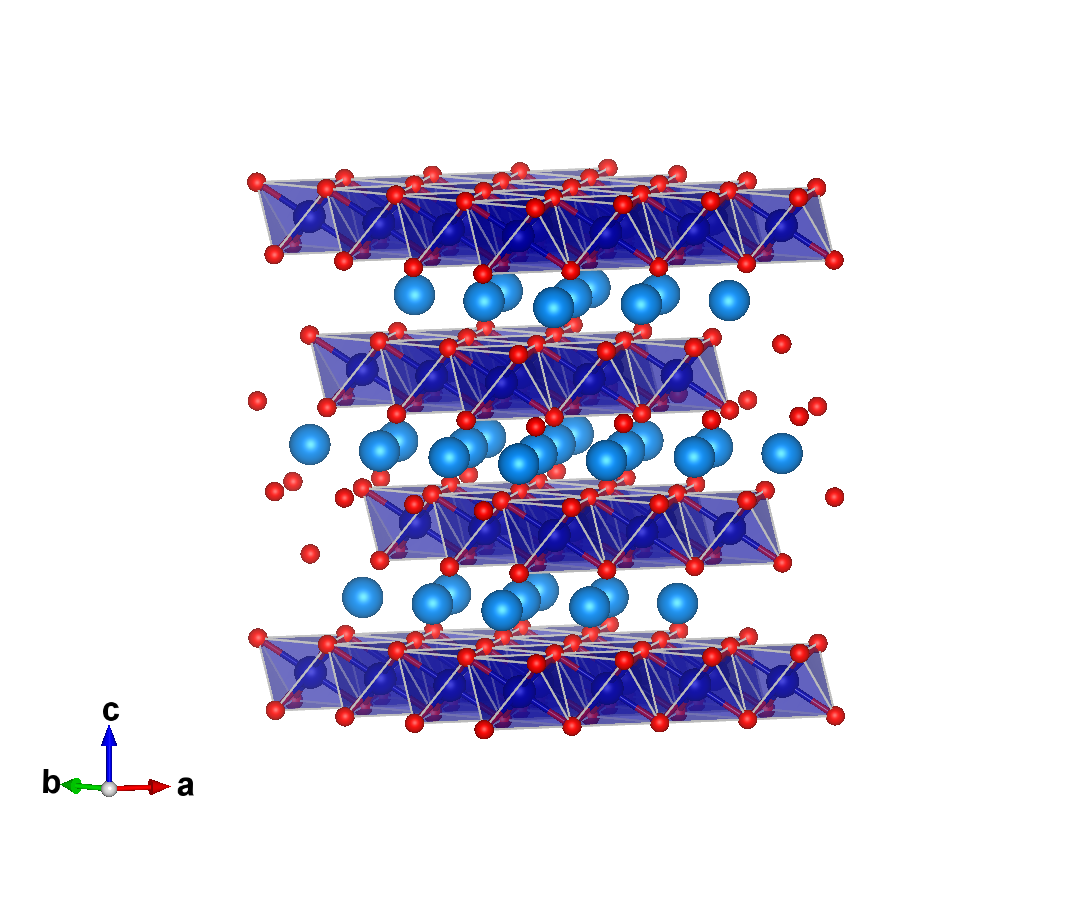
\includegraphics[width=0.18\textwidth]{CathodeMaterials/LiCoO2.png}\vspace{-1.0em}}
    &140&4,1&\cite{Zhang2004,Lyu2020}\\
    \ce{Li2NiO2}&\makecell{\vspace{-0.5em}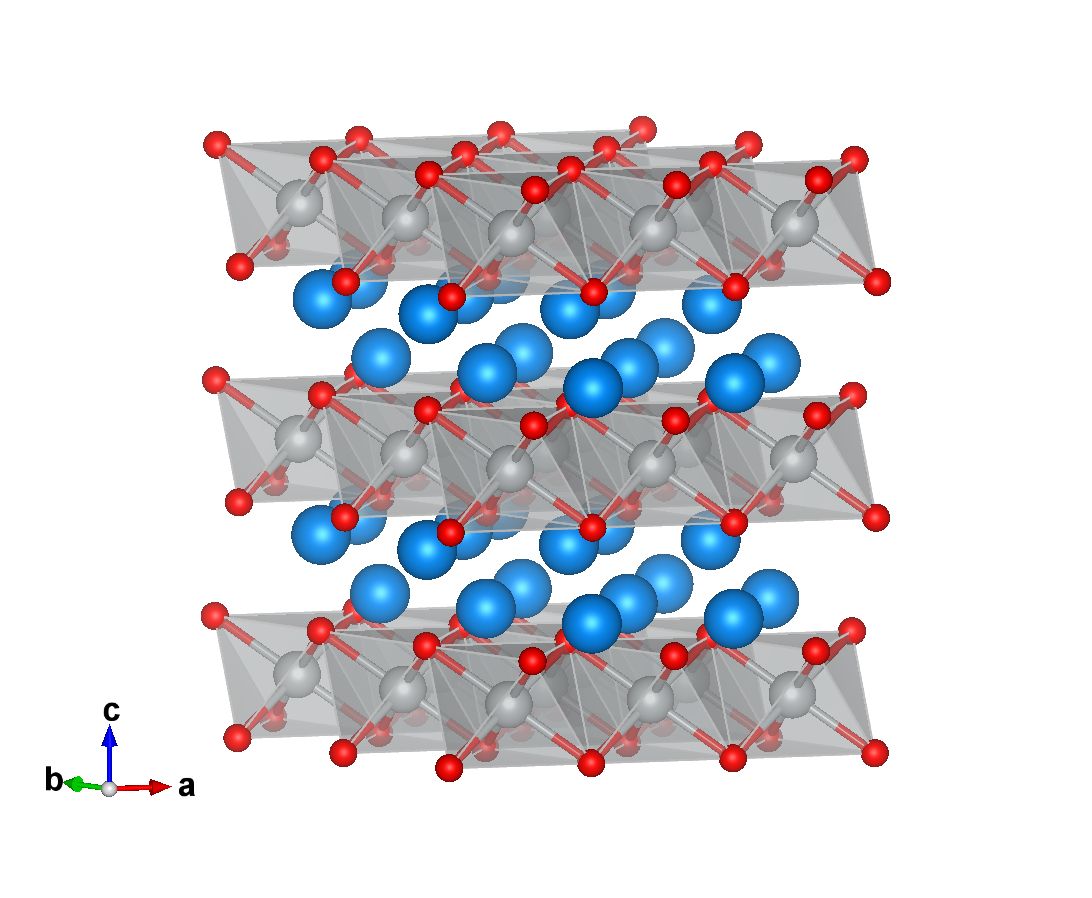
\includegraphics[width=0.18\textwidth]{CathodeMaterials/Li2NiO2.png}\vspace{-0.5em}}
    &235&4,0&\cite{Fan1998,Dahn1991,Arai1997}\\
    \ce{LiMnO2}&\makecell{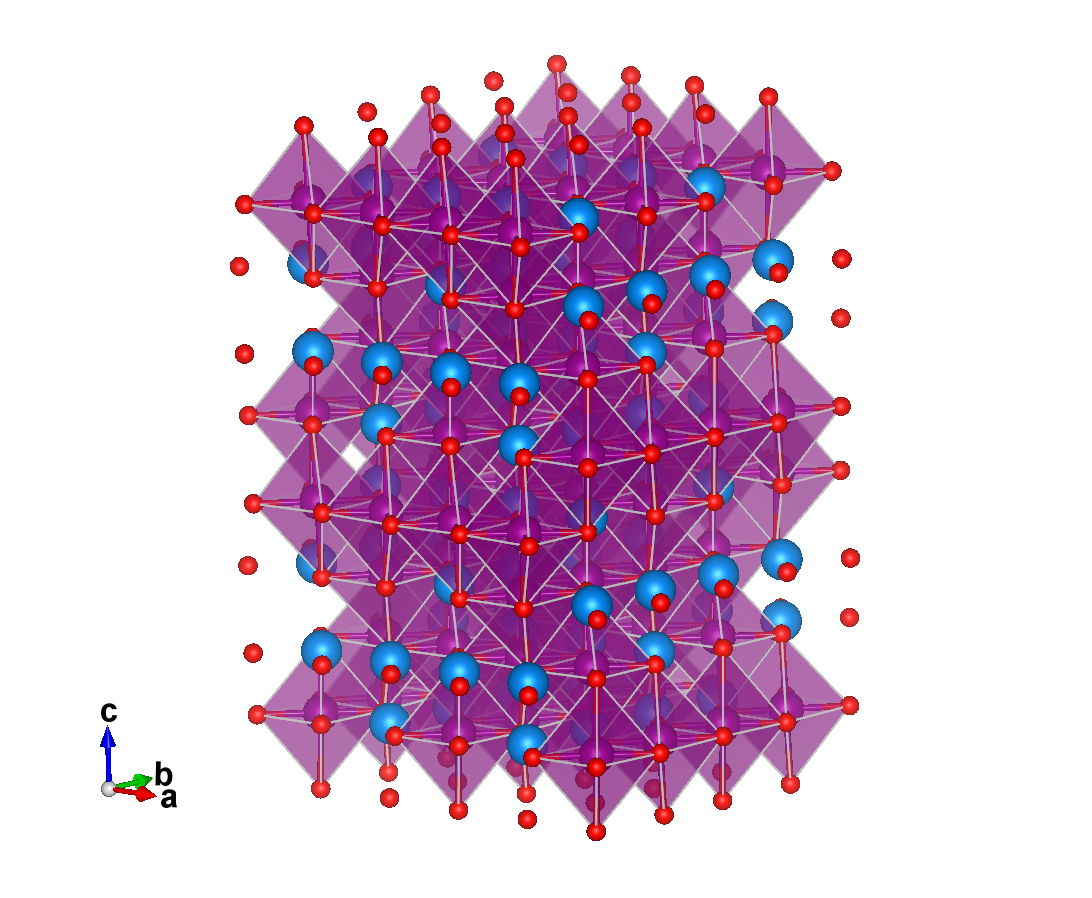
\includegraphics[width=0.18\textwidth]{CathodeMaterials/LiMnO2.png}\vspace{-0.8em}}
    &150&4,7&\cite{Croguennec1996,Vitins1997}\\
    \ce{LiFePO4}&\makecell{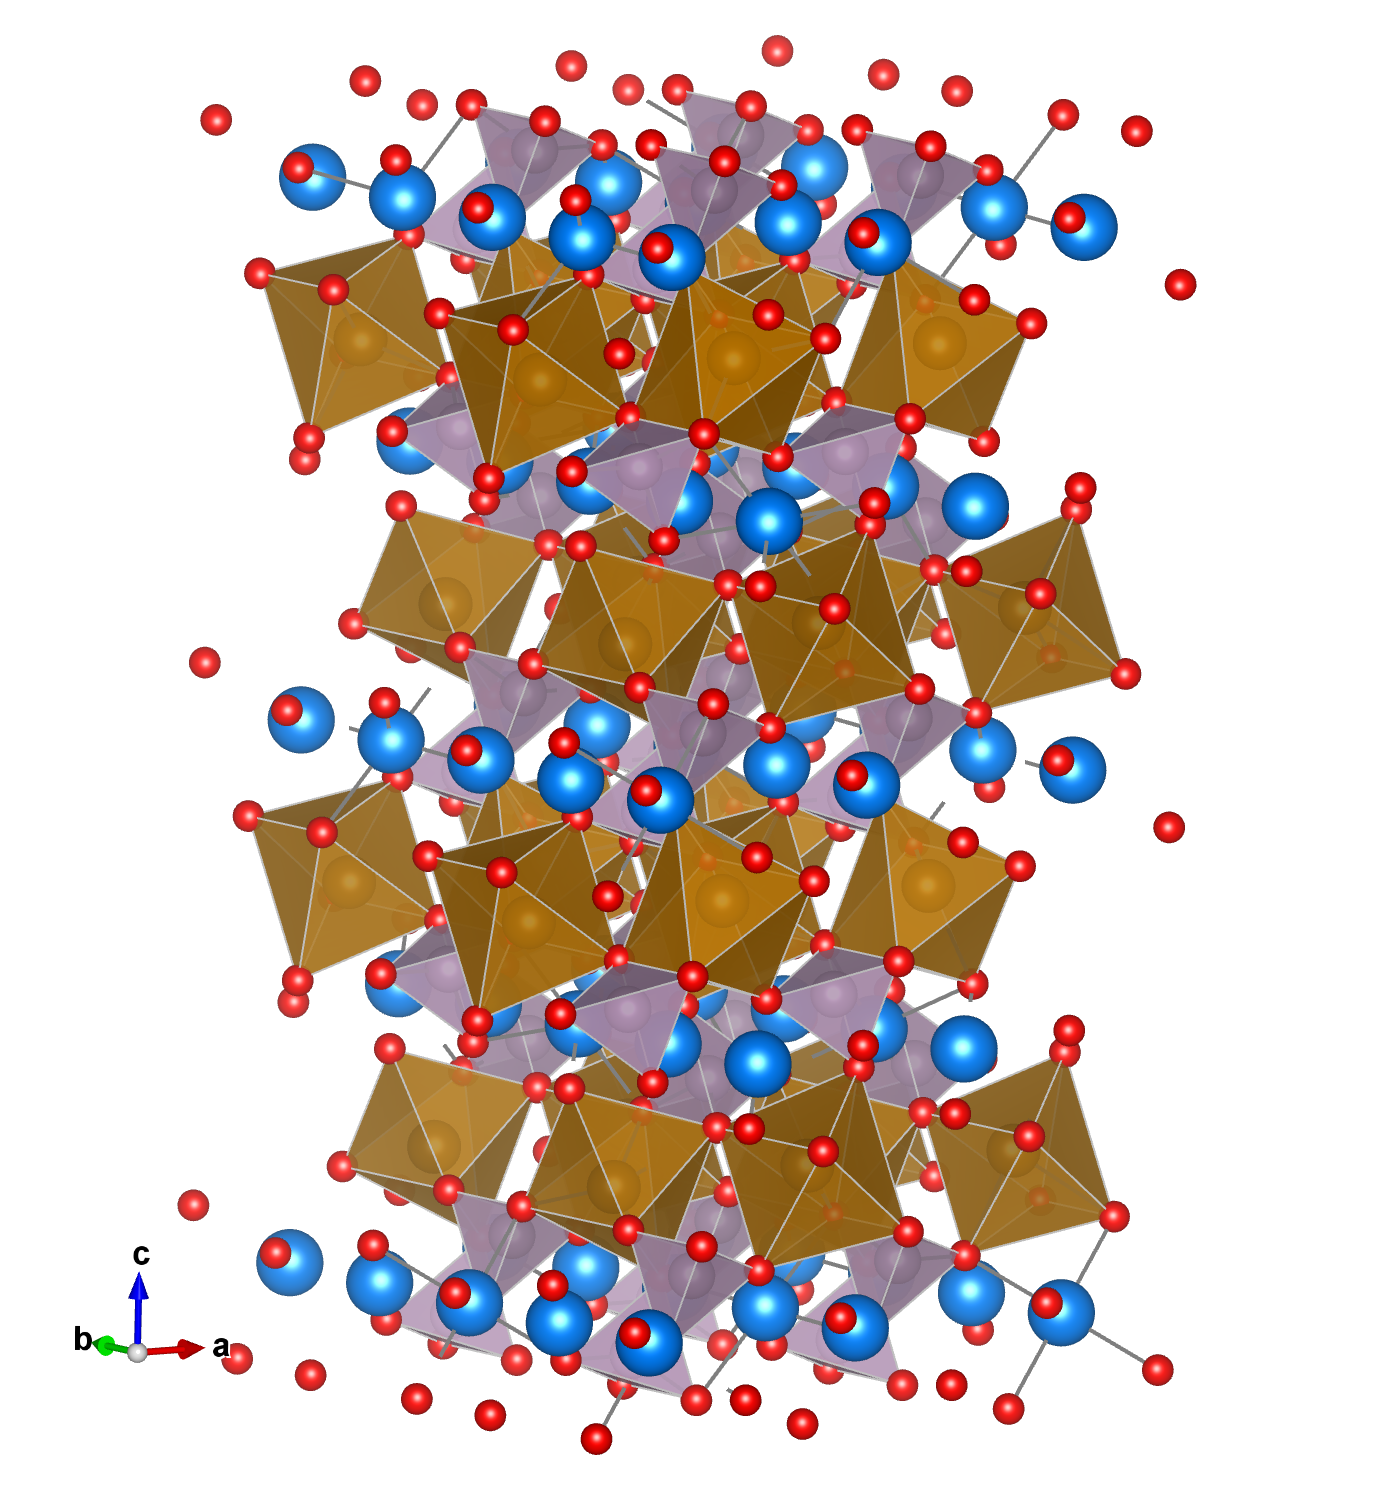
\includegraphics[width=0.18\textwidth]{CathodeMaterials/LiFePO4.png}\vspace{-0.8em}}
    &138&3,6&\cite{Padhi1997} \\
    \ce{LiNMC}111&\makecell{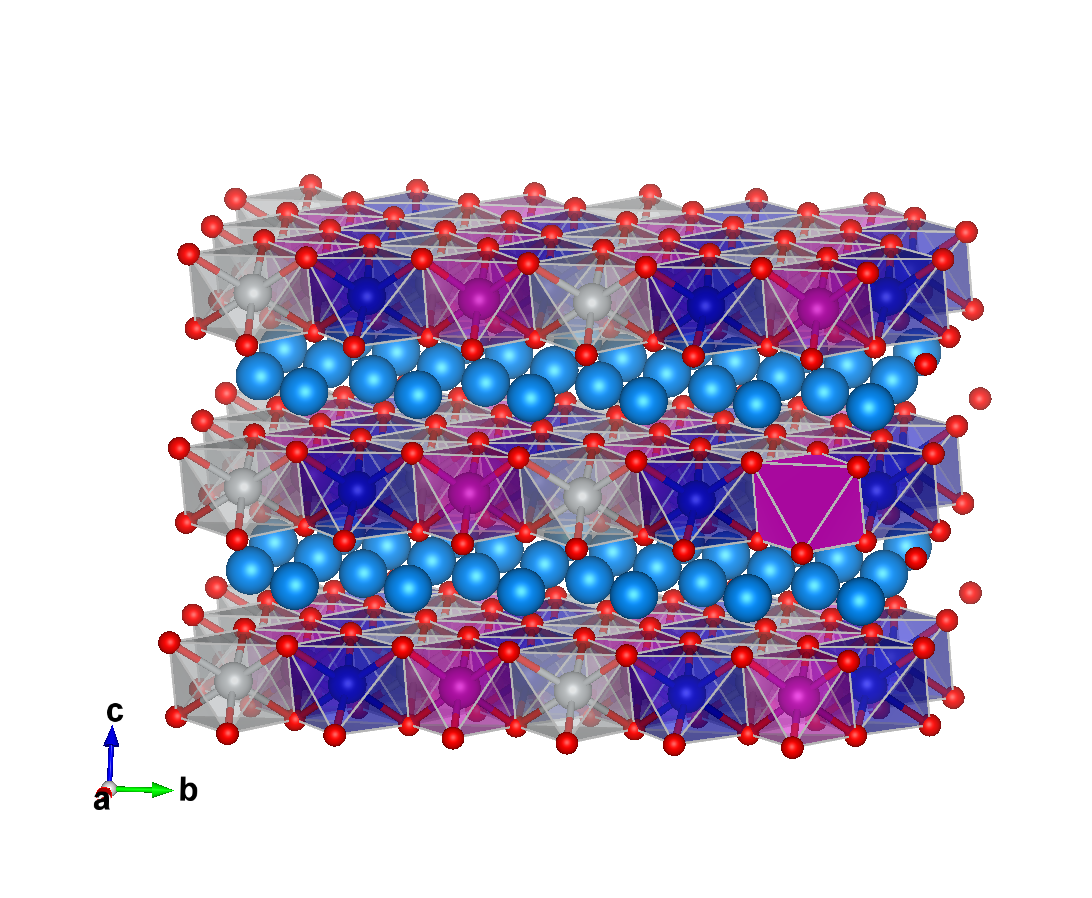
\includegraphics[width=0.18\textwidth]{CathodeMaterials/LiNMC111.png}\vspace{-0.5em}}
    &145&4,5&\cite{Park2024,Schmiegel2019}\\
    \ce{LiNMC}811&\makecell{\includegraphics[width=0.18\textwidth]{CathodeMaterials/LiNMC811.png}\vspace{-0.7em}}
    &230&4.3&\cite{Bhowmik2025,Quilty2024}\\
    \bottomrule
    \end{tabular}\\
    \noindent{\footnotesize{\textsuperscript{*} Gemessen gegenüber \ce{Li}/\ce{Li+}.}}
\end{table}%